\chapter{Forced Vibrations \& Resonance}


	In this chapter, we consider the effects of a \textbf{driving force} $F(t)$ on a system:
	\[ {F(t) = F_0 \cos(\omega t)} \]
	where...
	\begin{itemize}
		\item $\omega$ represents the \textbf{driving frequency}
		\item $\omega_0$ represents the \textbf{natural frequency} of the system, associated with a \textbf{free vibration} (see Chapter~\ref{ch:free-vibrations})
	\end{itemize}



We will see that...
\begin{itemize}
	\item As $\omega \to \omega_0$, the amplitude of oscillation increases
	\item ... whereas as $\omega$ gets farther away from $\omega_0$, the amplitude becomes smaller
	\item This phenomenon is known as \textbf{resonance}.
\end{itemize}

The system will initially have the tendency to vibrate at $\omega_0$, but it will ultimately begin to vibrate at $\omega$. We thus have two stages:
\begin{enumerate}
	\item \textbf{Transient state}: we have a superposition of oscillations at frequencies $\omega$ and $\omega_0$. The free vibration gradually gets damped away until...
	\item \textbf{Steady state}: only the the driving vibration remains, so the system oscillates at $\omega$
\end{enumerate}

\section{Forced Oscillations without Damping: Steady State}
We will consider the \emph{steady state} of a forced oscillation with \emph{negligible damping}, ignoring the fact that we need damping to get past the transient state.

Force equation:
\begin{align}
	m\ddot{x} &= -kx + F_0 \cos(\omega t)  \notag \\
	\Longrightarrow
	\mcol{m}\ddot{x} + \kcol{k}x &= F_0 \cos(\omega t)	\label{ch4:eq-no-b}
\end{align}

The behaviour or the system is illustrated in Figure~\ref{ch4:no-damping-pendula}.

\begin{figure}
	\centering
	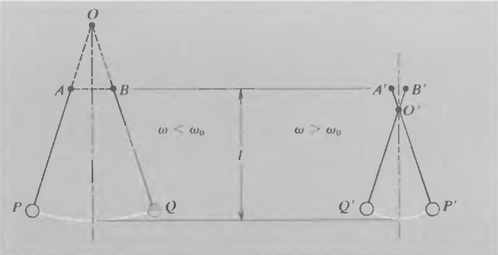
\includegraphics[scale=0.6]{phys232/Ch4-forced-no-damping-pendula.png} 
	\caption{The motion of simple pendula undergoing horizontal forced oscillations when (a) $\omega<\omega_0$ and (b) $\omega>\omega_0$.}\label{ch4:no-damping-pendula}
\end{figure}

\paragraph{Case (a): $\omega < \omega_0$}
If the driving force's frequency is much lower than the natural frequency...
\begin{itemize}
	\item We expect a low acceleration (since $\ddot{x} \propto \omega^2$).
	\item So, the $\kcol{k}x$ term dominates over $\mcol{m}\ddot{x}$; i.e. the response is controlled by the \kcol{stiffness} of the string.
	\item The phase delay between the driving force and the displacement is $\alpha=0$.
	\item Thus, $F_0 \approx kA$, and the amplitiude will be $A\approx F_0/k$
\end{itemize}

\begin{marginfigure}
	\normalsize
	\begin{tabular}{ccc}
		\hline
		Case & $A$ & {$\alpha$}  \\
		\hline
		$\omega < \omega_0$ & large & 0° \\
		$\omega > \omega_0$ & small & 180° \\
		\hline \\
	\end{tabular}
	\caption{Summary of cases~(a) and (b). Note that $\alpha$ represents the phase difference by which the driving force \emph{leads} the displacement.}
\end{marginfigure}

\paragraph{Case (b): $\omega > \omega_0$}
If the driving force's frequency is much higher than the natural frequency...
\begin{itemize}
	\item We expect a higher acceleration (since $\ddot{x} \propto \omega^2$).
	\item So, the $\mcol{m}\ddot{x}$ term dominates over $\kcol{k}x$; i.e. the response is controlled by the \mcol{inertia} of the string.
	\item We expect a relatively small $A$, opposite in phase with the driving force -- i.e. the driving force leads the displacement by a phase difference of $\alpha=180$.%
	\footnote{Notice that in Figure~\ref{ch4:no-damping-pendula}b, when $F$ is to the left, $x$ is to the right; when $F$ is to the right, $x$ is to the left.}
\end{itemize}




\subsection{Responant response ($\omega = \omega_0$)}

We will now examine why the we obtain a much higher amplitude (the \textbf{resonant amplitude}) when $\omega = \omega_0$.

Assume we are in the steady state; i.e. the natural oscillations are not present. Hence:
\begin{align}
	x &= C\cos(\omega t) \notag \\
	\Longrightarrow
	\ddot{x} &= -\omega^2 C\cos(\omega t)	\label{ch4:eq-acc-forced-no-b}
\end{align}

Substitute \eqref{ch4:eq-acc-forced-no-b} into \eqref{ch4:eq-no-b}:
\begin{align*}
	-m\omega^2 C\cancel{\cos(\omega t)} + kC\cancel{\cos(\omega t)} &= F_0\cancel {\cos(\omega t)} \\
	C(k-m\omega^2) &= F_0
\end{align*}
\begin{equation*}
	 C = \frac{F_0}{k-m\omega^2} = \frac{F_0/m}{\omega_0^2-\omega^2} 
\end{equation*}

To avoid working with negative values of $C$, let $A=|C|$. Use $\alpha$ again to represent the phase difference by which the driving force leads $x$.
\begin{equation*}
	\therefore
	x = A \cos(\omega t + \alpha) 
\end{equation*}
where
\begin{equation}
	\boxed{
	\alpha = 
	\begin{cases}
		0 & \text{if } \omega<\omega_0 \\
		\pi & \text{if } \omega>\omega_0
	\end{cases}
	\andd
	A = \left| \frac{F_0/m}{\omega_0^2-\omega^2}  \right| 
	}
	\label{ch4:soln-no-b}
\end{equation}


\begin{marginfigure}
	\centering
	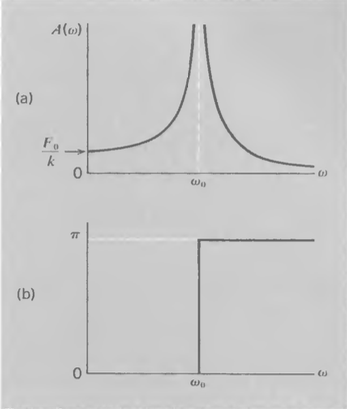
\includegraphics[scale=0.5]{phys232/Ch4-forced-no-damping-A.png} \caption{(a) Absolute amplitude of forced oscillations (no damping) as a function of $\omega$; (b) phase lag of $x$ with respect to the driving force, as a function of $\omega$.}	\label{ch4:no-damping-A}
\end{marginfigure}

The results in \eqref{ch4:soln-no-b} are plotted in Figure~\ref{ch4:no-damping-A}. Notice that as $\omega\to\omega_0$, $C\to \infty$.


\subsection{Resonant response, using complex exponentials}
Recall \eqref{ch4:eq-no-b}:
\[ m\ddot{x} + kx = F_0 \cos(\omega t) \]

Visualize the driving force $F_0 \cos(\omega t)$ as the real component of $F_0 e^{j\omega t}$.

Assume $x$ is the real part of a rotating vector $z$, such that:
\[ m\ddot{z} + kz = F_0 e^{j\omega t}\]

Assume the following solution:
\[z = Ae^{j(\omega t+\alpha)} \]

Substitute in \eqref{ch4:eq-acc-forced-no-b}:
\begin{align*}
	(-m\omega^2 A + kA)e^{j(\cancel{\omega t} + \alpha)} &= F_0 \, \cancel{e^{j\omega t}} \\
	A(-\omega^2 + \omega_0^2)e^{j\alpha} &= \frac{F_0}{m} \\
	A(\omega_0^2 - \omega^2 ) &= \frac{F_0}{m} e^{-j\alpha} \\
	\Longrightarrow
	\underbrace{A(\omega_0^2 - \omega^2 )}_\text{real} &= \underbrace{\frac{F_0}{m} \cos\alpha}_\text{real} - \underbrace{j\frac{F_0}{m} \sin\alpha}_\text{imaginary}
\end{align*}

Comparing the real and imaginary components on each side:
\begin{align*}
	\text{Real part: } \htab & A(\omega_0^2 - \omega^2 ) = \frac{F_0}{m} \cos\alpha \\
	\text{Imaginary part: } \htab & \frac{F_0}{m} \sin\alpha = 0 
\end{align*}

From the imaginary part, $\alpha = n\pi, n\in\mathbb{Z}$. Thus, $\cos\alpha=0$ in the real part, and we obtain:
\begin{align*}
	A(\omega_0^2 - \omega^2 ) &= \frac{F_0}{m} \\
	\therefore
	A &= \frac{F_0/m}{\omega_0^2 - \omega^2 }
\end{align*}

... which is the same result as \eqref{ch4:soln-no-b}.

\section{Forced Oscillations with Damping: Steady State}

Let us continue to examine only the \emph{steady state}.

Equation of motion:
\[ \ddot{x} + \gamma\dot{x} + \omega_0^2 = F_0 \cos(\omega t) \]

Results: 
\[ x = A \cos (\omega t - \delta) \]
\[ A(\omega) = \frac{F_0/m}{[(\omega_0^2 - \omega^2)^2 + (\gamma\omega)^2]^{1/2}} \]
\[ \tan \delta (\omega) = \frac{\gamma\omega}{\omega_0^2 - \omega^2}\]

Independent of adjustable initial starting conditions!

\subsection{Transient Effects}
For $t<0$, let the object be at rest (i.e. it only starts moving at $t=0$).
\begin{align*}
x &= steady + transient \\
x &= A \cos (\omega t - \delta) + B e^{-\gamma t/2} \cos(\omega' + \beta)
\end{align*}

The transient part (system's ''natural" motion) dies out over time due to damping; after then, the steady state takes over. 

Transient part of the equation accounts for adjustable initial conditions!

A \emph{beat pattern} may be produced during this stage if $\omega'$ (system's freq w/ damping) and $\omega$ are similar.

\section{Power}
Power required to keep a driven oscillator going at the same amplitude:
\[ P = \frac{dW}{dt} = F\frac{dx}{dt} = Fv \]